\title{Syllabus for Algebra-Based Physics 1 (Mechanics): PHYS135A}
\author{Dr. Jordan Hanson - Whittier College Dept. of Physics and Astronomy}
\date{\today}
\documentclass[10pt]{article}
\usepackage[margin=1.5cm]{geometry}
\usepackage{outlines}
\usepackage{hyperref}
\usepackage{graphicx}
\begin{document}
\maketitle

\begin{abstract}
The concepts of algebra-based mechanics will be presented via interactive problem-solving in an integrated lecture/laboratory format.  First, the concepts of displacement, velocity, and acceleration in one and two dimensions will be introduced, building up to Newton's Laws of motion.  Next, the concepts of friction and rotational motion will be added.  More complex problems will be introduced through the conservation of energy and linear momentum, followed by the rotational equivalents.  This course includes analytic textbook problems, peer instruction and group discussions, interactive computational exercises, and lab-based activities.
\end{abstract}
\noindent
\textit{\textbf{Pre-requisites}: None} \\
\textit{\textbf{Course credits, Liberal Arts Categorization}: 4 Credits, None} \\
\textit{\textbf{Regular course hours and location}: Monday and Wednesday, 8:50 am - 10:50 am, SLC 232.} \\
\textit{\textbf{Instructor contact information}: jhanson2@whittier.edu (email), 918particle (Discord).} \\
\textit{\textbf{Office hours}: Please use the following link to schedule meetings: \url{https://fgucmvjkylvmgqfsco.10to8.com}.} \\
\textit{\textbf{Attendance/Absence}: Students needing to reschedule midterms must notify the professor a few days in advance.} \\ 
\textit{\textbf{Late work policy}: Late work is generally not accepted, but is left to the discretion of the instructor.} \\
\textit{\textbf{Course texts}: College Physics, 2nd ed., (OpenStax).  This course text is free and open-access: \url{https://openstax.org/details/books/college-physics-2e}.} \\
\textit{\textbf{Grading}: The course grade will be a weighted average of assignment scores, and the weights are listed in Tab. \ref{tab:grades}.}
\begin{table}
\centering
\begin{tabular}{| c | c | c |}
\hline
\textbf{Assignment} & \textbf{Weight} & \textbf{Date} \\ \hline
Daily exercises & 10 \% & Mondays and Wednesdays, 8:50 am - 10:50 am\\ \hline
Homework sets and labs & 30 \% & Fridays, submitted online using ExpertTA \\ \hline
First Midterm Exam & 20 \% & October 14th, 2024 (take-home style on Units 0-3) \\ \hline
Second Midterm Exam & 20 \% & December 9th, 2024 (take-home style on Units 4-8) \\ \hline
Final Project Presentation & 20\% & December 2nd and 4th, 2024 (in class) \\ \hline
\end{tabular}
\caption{\label{tab:grades} These are the grade weights for each assignment. The final project presentation can take two forms.  \textbf{Option A}: A 10-15 minute traditional presentation with several minutes for questions.  \textbf{Option B}: A video in digital storytelling format using WeVideo, also 10-15 minutes long.}
\end{table}
\noindent
\textit{\textbf{Grade Settings}: $\geq 60\%, <70\%$ = D, $\geq 70\%, <80\%$ = C, $\geq 80\%, <90\%$ = B, $\geq 90\%, <100\%$ = A. Pluses and minuses: 0-3\% minus, 3\%-6\% straight, 6\%-10\% plus (e.g. 79\% = C+, 91\% = A-).} \\
\textit{\textbf{ADA Statement on Disability Services}: Whittier College is committed to make learning experiences as accessible as possible. If you experience physical or academic barriers due to a disability, you are encouraged to contact Student Disability Services (SDS) to discuss options. To learn more about academic accommodations, email disabilityservices@whittier.edu, call (562) 907-4825, or go to SDS which is located on the ground floor of Wardman Library.} \\
\textit{\textbf{Academic Honesty:} \url{https://www.whittier.edu/policies/academic/honesty}} \\
\noindent
\textit{\textbf{Course Objectives}:}
\begin{itemize}
\item Develop skill in written and oral expression of technical ideas.
\item Improve performance in solving technical problems using physics and mathematics.
\item Develop skill in constructing mathematical models of mechanical systems.
\item Improve performance in the application of conceptual and logical thinking in technical scenarios.
\item To practice scientific experimentation, data analysis, and reporting of results.
\end{itemize}
\clearpage
\twocolumn
\noindent
\textit{\textbf{Course Outline}:}
\begin{outline}[enumerate]
\1 \textbf{Unit 0:} Review and preparation 
\2 Course introduction and organization, peer instruction modality
\2 Physical science review - \textbf{Chapters 1.1 - 1.4}
\3 Physical quantities
\3 Estimation and unit analysis
\2 Kinematics, I - \textbf{Chapters 2.1 - 2.4}
\3 Distance, velocity, and time
\2 \textit{Problem sets:}
\3 \textit{Problem set 1: chapters 1.1 - 1.4}
\3 \textit{Problem set 2: chapters 2.1 - 2.4}
\1 \textbf{Unit 1:} One and two-dimensional kinematics
\2 Kinematics, II - \textbf{Chapters 2.5 - 2.8}
\3 Definitions of time, displacement, velocity, acceleration
\3 Kinematic equations with constant acceleration
\2 Kinematics, III - \textbf{Chapters 3.1 - 3.4}
\3 Definition of vector quantities, vector addition and subtraction
\3 Kinematics in more than one dimension
\3 Graphical analysis applied to kinematics
\3 Projectile motion
\2 \textit{Problem sets:}
\3 \textit{Problem set 3: chapters 2.5 - 2.8}
\3 \textit{Problem set 4: chapters 3.1 - 3.4}
\1 \textbf{Unit 2:} Forces and Newton's Laws
\2 Forces, I - \textbf{Chapters 4.1 - 4.4}
\3 Definition of force, free-body diagrams
\3 Newton's First Law
\3 Newton's Second Law
\3 Newton's Third Law
\2 Forces, II: applications - \textbf{Chapters 4.5 - 4.7}
\3 Normal forces, tension, other examples
\2 \textit{Problem sets:}
\3 \textit{Problem set 5: chapters 4.1 - 4.4}
\1 \textbf{Unit 3:} Applications of Newton's Laws
\2 Forces, III: applications - \textbf{Chapters 4.5 - 4.7}
\3 Friction
\3 Drag forces
\2 Forces, IV: applications - \textbf{Chapters 5.1 - 5.3}
\3 Elasticity and Young's modulus
\3 Shear and strain, bulk modulus \\ \\
\2 \textit{Problem sets:}
\3 \textit{Problem set 6: chapters 4.5 - 4.7}
\3 \textit{Problem set 7: chapters 5.1 - 5.3}
\1 \textbf{First Midterm} - due October 14th, 2024
\2 The midterm will be posted on Moodle on Friday, October 11th.
\2 The exam will be completed at home, with an open-book/open-note policy.  The format includes multiple choice, written exercises, and design problems.
\2 The exam is due in PDF form on Monday, October 14th, to be submitted via Moodle.
\1 \textbf{Unit 4:} Rotational kinematics
\2 Uniform circular motion, I - \textbf{Chapters 6.1 - 6.3}
\3 Angular displacement, velocity, and acceleration
\3 Kinematic equations for rotation
\3 Centripetal force
\2 Gravity and Kepler's Laws - \textbf{Chapters 6.5 - 6.6}
\3 Newton's Law of Gravity
\3 Law of Gravity applied near Earth's surface
\3 Kepler's Laws and the solar system
\2 \textit{Problem sets:}
\3 \textit{Problem set 8: chapters 6.1 - 6.3}
\3 \textit{Problem set 9: chapters 6.5 - 6.6}
\1 \textbf{Unit 5:} Work and Energy
\2 Energy, I - \textbf{Chapters 7.1 - 7.4}
\3 Scientific definition of work
\3 Kinetic energy and the work-energy theorem
\3 Potential energy
\2 Energy, II - \textbf{Chapters 7.6 - 7.8}
\3 Energy conservation and power
\3 Energy and power in human physiology
\2 \textit{Problem sets:}
\3 \textit{Problem set 10: chapters 7.1 - 7.4}
\3 \textit{Problem set 11: chapters 7.6 - 7.8}
\1 \textbf{Unit 6:} Linear momentum
\2 Momentum, I - \textbf{Chapters 8.1 - 8.3}
\3 Mathematics review: systems of equations
\3 Definition of linear momentum
\3 Momentum conservation
\2 Momentum, II - \textbf{Chapters 8.4 - 8.6}
\3 Elastic and inelastic scattering
\3 Scattering in more than one dimension
\3 \textit{Problem sets:}
\3 \textit{Problem set 12: chapters 8.1 - 8.3, 8.4 - 8.6}
\1 \textbf{Unit 7:} Statics
\2 Forces, V - \textbf{Chapters 9.1 - 9.4}
\3 Definition of torque
\3 Two stability conditions in a static system
\2 \textit{Problem sets:}
\3 \textit{Problem set 13: chapters 9.1 - 9.4}
\1 \textbf{Unit 8:} Rotational dynamics
\2 Uniform circular motion, II - \textbf{Chapters 10.1 - 10.4}
\3 Angular kinematics, II: displacement, velocity, and acceleration 
\3 Angular dynamics: force and torque
\3 Rotational kinetic energy
\2 Angular momentum - \textbf{Chapter 10.5}
\2 \textit{Problem sets:}
\3 \textit{Problem set 14: chapters 10.1 - 10.4, 10.5}
\1 \textbf{Second Midterm} - due December 9th, 2024
\2 The midterm will be posted on Moodle on Friday, December 6th.
\2 The exam will be completed at home, with an open-book/open-note policy.  The format includes multiple choice, written exercises, and design problems.
\2 The exam is due in PDF form on Monday, December 9th, to be submitted via Moodle.
\1 \textbf{Final project presentations}
\2 Presented via option A or B (see Tab. \ref{tab:grades}).
\2 Given on December 2nd and 4th
\2 Project teams can be groups of 2-3
\2 Teams will complete a self-designed and self-constructed DIY physics experiment
\2 \textbf{Option A}: A 10-15 minute traditional presentation with several minutes for questions.
\2 \textbf{Option B}: A video in digital storytelling format using WeVideo, also 10-15 minutes long.
\2 Students will receive training and access for the WeVideo tools, which Whittier College provides for free.
\2 Presentations will be graded according to the following breakdown:
\3 For presenting results emphasizing \textit{precision and attention to detail}, with \textit{experimentally verifiable} content, 30\%.
\3 For \textit{clearly communicating} the content, including legibility and sensible graphics, 30\%.
\3 For \textit{meeting but not exceeding} the time-requirement with appropriate amount of content, 30\%.
\3 For \textit{articulating the idea with a unique style}, 10\%.
\end{outline}
\begin{figure}[ht]
\centering
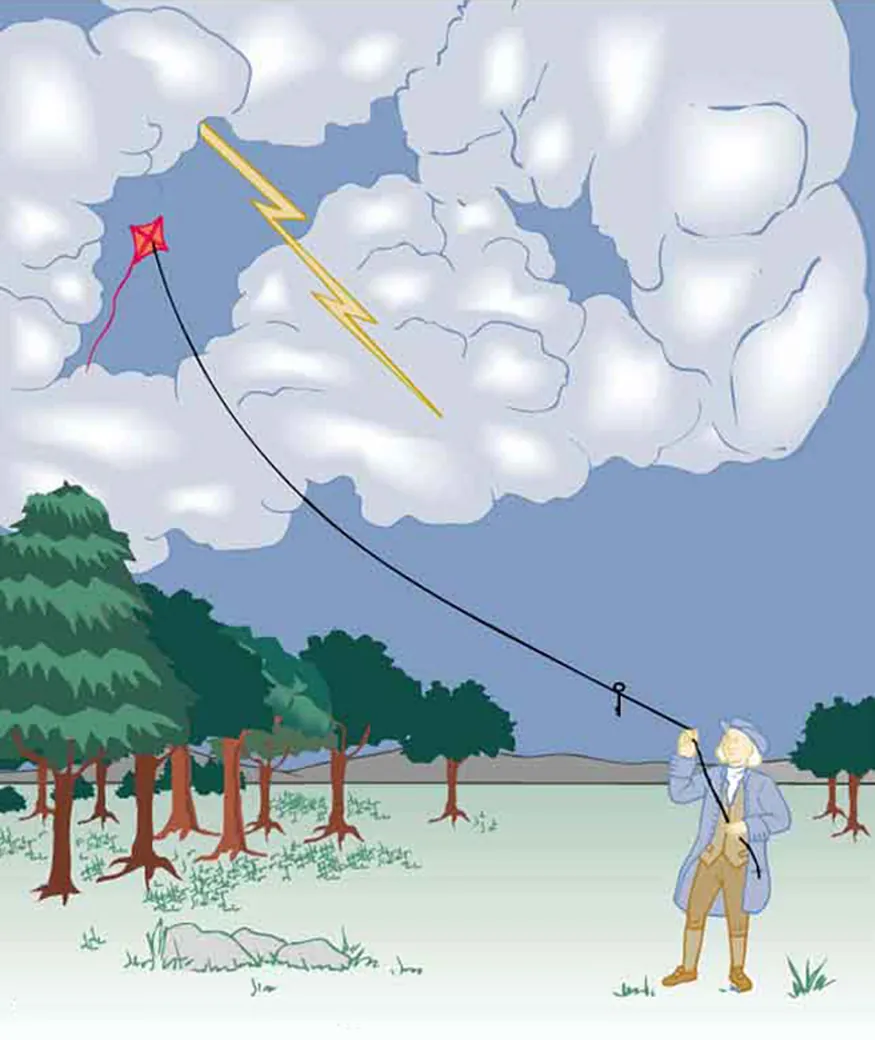
\includegraphics[width=0.15\textwidth]{figures/franklin.png}
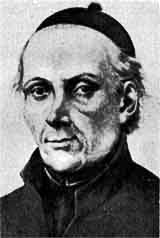
\includegraphics[width=0.15\textwidth]{figures/alzate_ramirez.jpg} \\
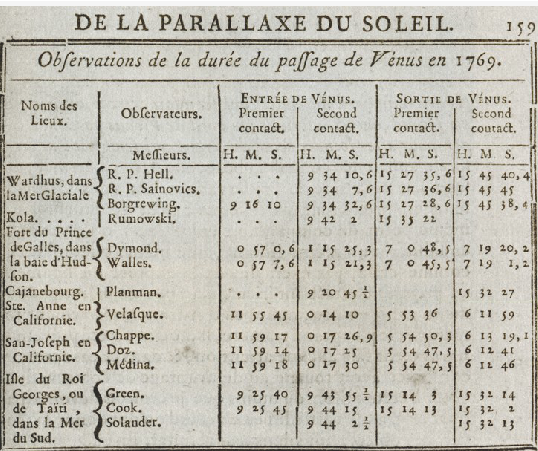
\includegraphics[width=0.30\textwidth]{figures/1769_transit.png} \\
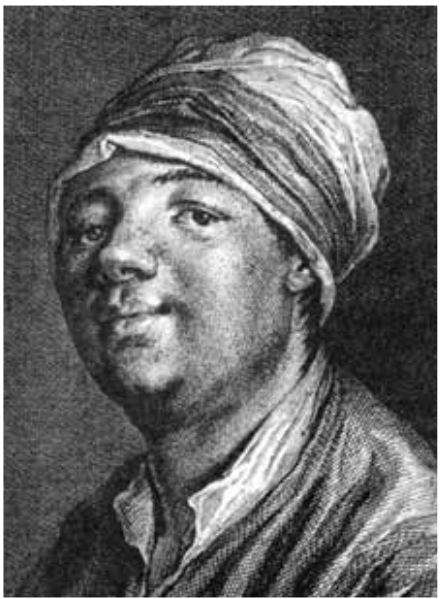
\includegraphics[width=0.15\textwidth]{figures/Abbot_dAuteroche.png}
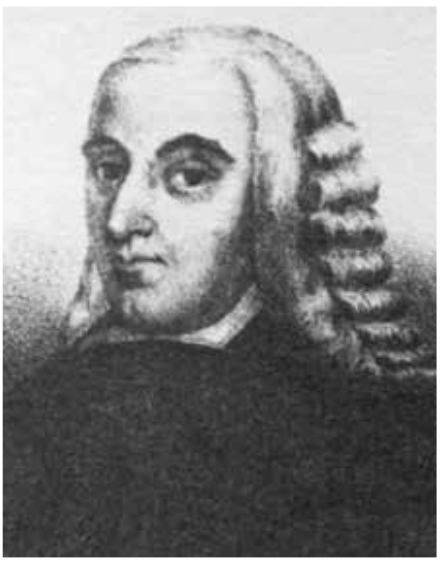
\includegraphics[width=0.15\textwidth]{figures/joaquin_v_d_Leon.png}
\caption{\label{fig:franklin} \small (Top left) Benjamin Franklin, (Top right) Father Jos\'{e} Antonio Alzate y Ram\'{i}rez, (Middle) Astronomical data from 1769 Venus transit, (Bottom left) Jean-Baptiste Chapp\'{e} d'Auteroche, (Bottom right) Joaqu\'{i}n Vel\'{a}zquez de Le\'{o}n.}
\end{figure}
\begin{figure}[hb]
\centering
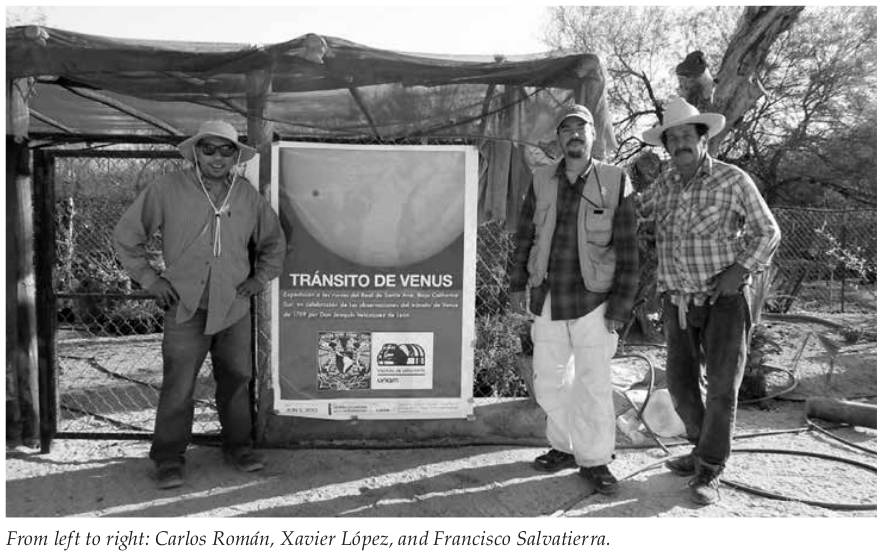
\includegraphics[width=0.375\textwidth]{figures/roman_lopez_salvatierra.png}
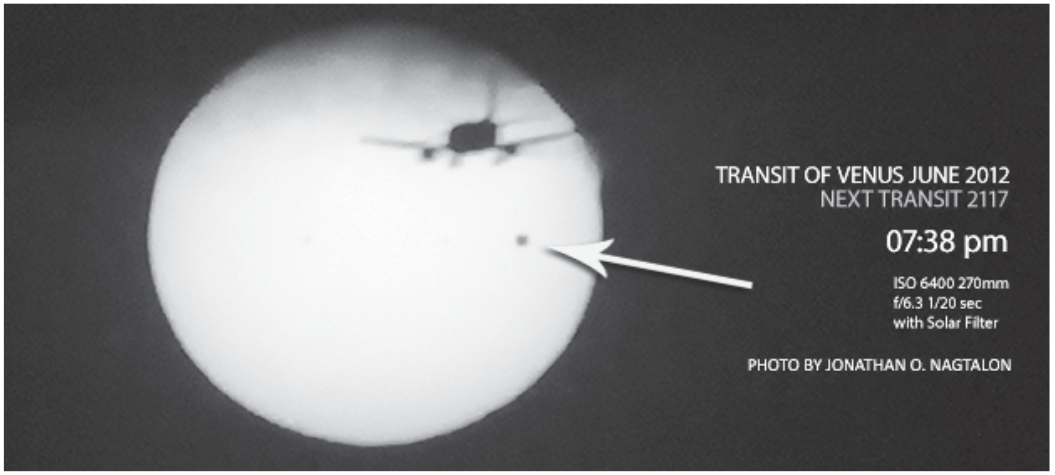
\includegraphics[width=0.375\textwidth]{figures/venus.png}
\caption{\label{fig:franklin2} \small (Top) Carlos Rom\'{a}n, Xavier L\'{o}pez, and Fransisco Salvatierra. (Bottom) The 2012 Venus transit, from Baja California.}
\end{figure}
\end{document}
